\documentclass[]{standalone}

\usepackage{tikz}
\usepackage{amsmath}
\usepackage{unicode-math}
\usepackage{xcolor}

\newcommand{\rvec}[1]{\mathbfit{#1}}

\usetikzlibrary{
  calc,
  arrows, arrows.meta,
  positioning, intersections,
  patterns, patterns.meta,
}
\tikzset{
  dot/.style = {circle, fill=red!80!gray, minimum
      size=#1, draw=black,
      inner sep=0pt, outer sep=0pt},
  dot/.default = 5pt, % size of the circle diameter 
  wdot/.style = {dot=#1, fill=white},
  wdot/.default = 5pt, % size of the circle diameter 
  bdot/.style = {dot=#1, fill=black},
  bdot/.default = 5pt, % size of the circle diameter 
}

\begin{document}
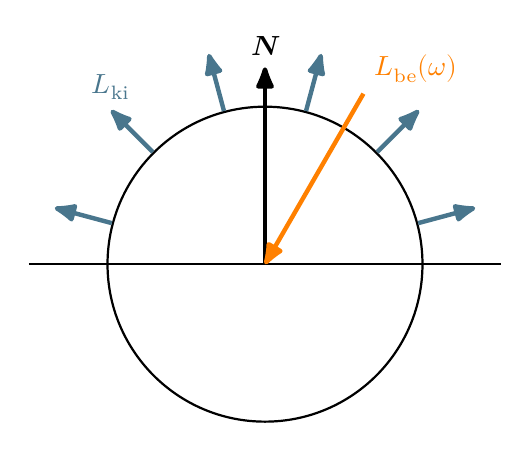
\begin{tikzpicture}[thick]
  \coordinate (o) at (0,0);

  \draw (-3,0) -- (3,0);
  \node[circle, minimum size=4cm, draw=black] (circ) at (o) {};

  \draw[-{Latex[round]}, ultra thick] (o) -- (0,2.5)
  node[above] {$\rvec N$};
  \draw[orange,{Latex[round]}-, ultra thick] (o) -- ++(60:2.5)
  node[above right] {$L_\text{be}(\omega)$};
  \foreach \d in {15, 45, 75, 105, 135, 165} {
  \draw[cyan!50!black, ultra thick, -{Latex[round]}] (circ.\d) -- ++(\d:.75)
  coordinate (\d);
  }
  \node[cyan!50!black, above] at (135) {$L_\text{ki}$};
\end{tikzpicture}
\end{document}
